\subsection{Motion of the quadrocopter}\label{chapter_BASICS}

Theoretically a quadrocopter has six degrees of freedom: 
\begin{enumerate}
		\item Moving in direction of x (forward, backward)
		\item Moving in direction of y (left, right)
		\item Moving in direction of z (up, down)
		\item Rotation around the x-axis, called 'Roll'
		\item Rotation around the y-axis, called 'Pitch'
		\item Rotation around the z-axis, called 'Yaw'
\end{enumerate}
Effectively there are only four degrees of freedom, because movement in direction of x and y is only a side-effect by gravity, like it is described in chapter \ref{chapter_EQUATIONS_OF_MOTION}. 
These four degrees of freedom are exemplified in the following.

\subsubsection{Thrust}
\begin{figure}[htbp]
	\centering
		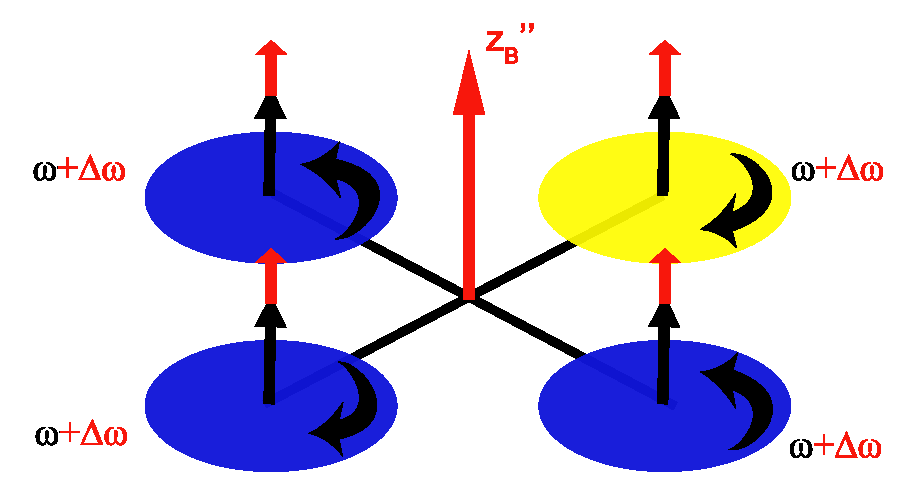
\includegraphics[width=0.7\textwidth]{03_Grafiken/Thrust.pdf}
	\caption{Thrust}
	\label{fig:Thrust}
\end{figure}

If all rotors are spinning with constant angular rate $\omega$ and a new offset $\Delta\omega$ is added, the ascending force of each rotor increases in same way, which results in a force vector, pointing in direction of z of the bodyframe. So the quadrocopter accelerates in direction of z.

\subsubsection{Pitch}
\begin{figure}[H]
	\centering
		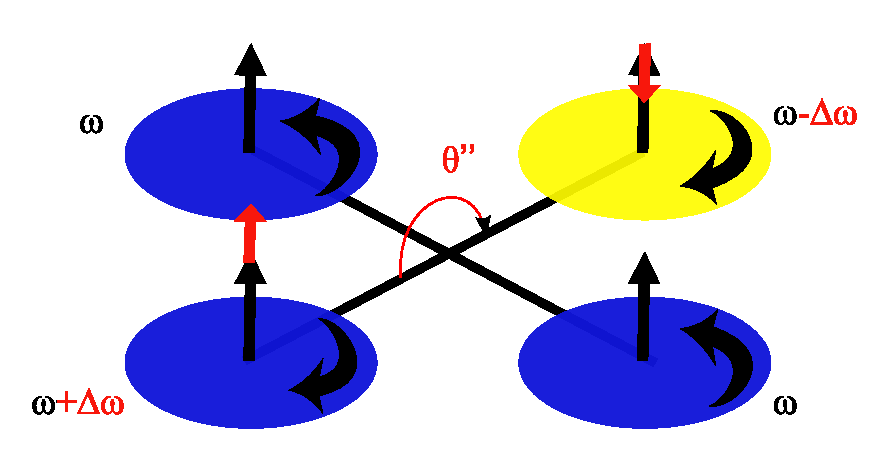
\includegraphics[width=0.7\textwidth]{03_Grafiken/Theta.pdf}
	\caption{Pitch}
	\label{fig:Theta}
\end{figure}
To achieve forward-pitching, the rotor in front is slowed down, what means a negative offset $\Delta\omega$. In addition a positive offset is added to the rear motor. The result is a change of the angular acceleration and therefore a change of the angle $\theta$ (theta).

\subsubsection{Roll}
\begin{figure}[htbp]
	\centering
		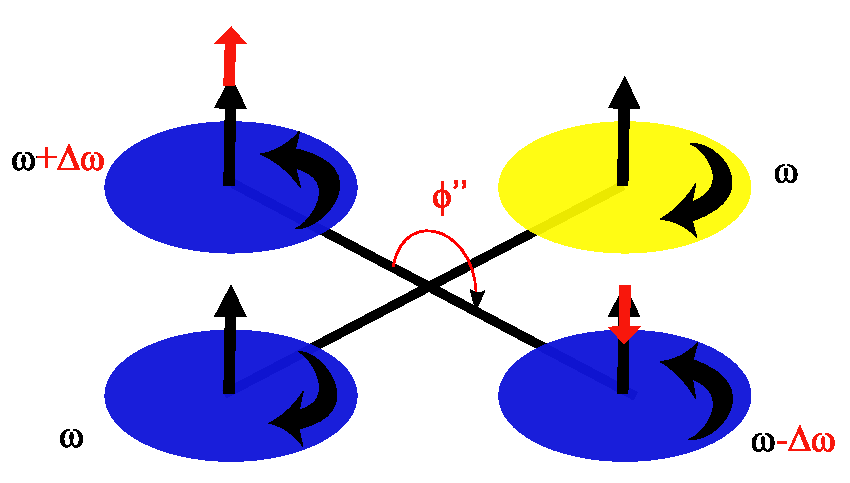
\includegraphics[width=0.7\textwidth]{03_Grafiken/Phi.pdf}
	\caption{Roll}
	\label{fig:Phi}
\end{figure}
The principle to get a roll movement is the same one, like it is used for the pitch movement. To achieve a roll movement to the right, a negative offset $\Delta\omega$ is added to the rotor on the right side of the quadrocopter. In addition a positive offset is added to the left rotor. Again the result is a change of the angular acceleration and therefore a change of the angle $\Phi$(phi)

\subsubsection{Yaw}
\begin{figure}[htbp]
	\centering
		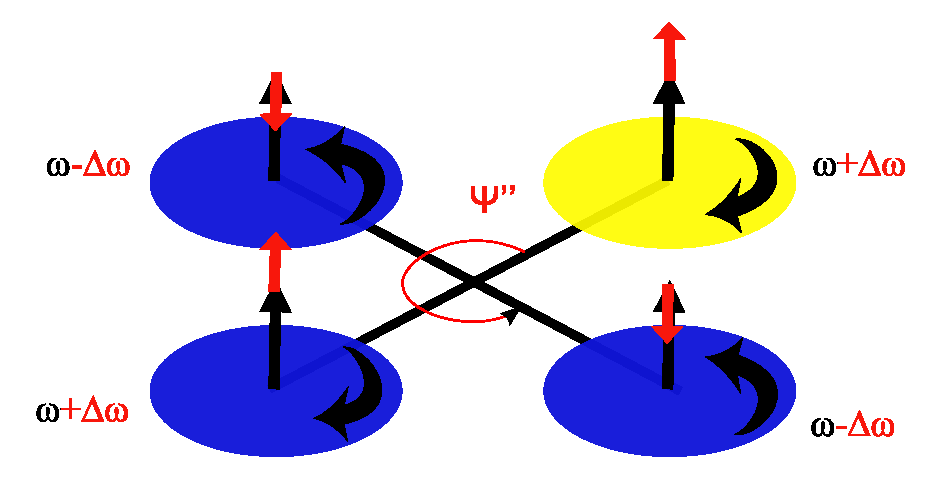
\includegraphics[width=0.7\textwidth]{03_Grafiken/Psi.pdf}
	\caption{Yaw}
	\label{fig:Psi}
\end{figure}
To achieve rotation around the z-axis, called 'yaw' is more tricky than the roll and pitch movements.
It is visible in the grapics, that the rotors at the front and the back of the quadrocopter spin clockwise, while the two rotors on the side of the quadrocopter spin counterclockwise. This is necessary because of the inertia of the propellers. If all propellers would spin clockwise, the quadrocopter would steadily rotate counterclockwise. This effect is used, to rotate the quadrocopter.
To achieve a rotation counterclockwise, a positive offset is added to the front rotor and the rear rotor. To intensify this effect and avoid thrust, the left and the right rotor, which hold up, are slowed down by adding a negative offset to their motor speed. The result is a vertical, counterclockwise rotation $\Psi$(psi).